% Options for packages loaded elsewhere
% Options for packages loaded elsewhere
\PassOptionsToPackage{unicode}{hyperref}
\PassOptionsToPackage{hyphens}{url}
\PassOptionsToPackage{dvipsnames,svgnames,x11names}{xcolor}
%
\documentclass[
  letterpaper,
  DIV=11,
  numbers=noendperiod]{scrartcl}
\usepackage{xcolor}
\usepackage{amsmath,amssymb}
\setcounter{secnumdepth}{-\maxdimen} % remove section numbering
\usepackage{iftex}
\ifPDFTeX
  \usepackage[T1]{fontenc}
  \usepackage[utf8]{inputenc}
  \usepackage{textcomp} % provide euro and other symbols
\else % if luatex or xetex
  \usepackage{unicode-math} % this also loads fontspec
  \defaultfontfeatures{Scale=MatchLowercase}
  \defaultfontfeatures[\rmfamily]{Ligatures=TeX,Scale=1}
\fi
\usepackage{lmodern}
\ifPDFTeX\else
  % xetex/luatex font selection
\fi
% Use upquote if available, for straight quotes in verbatim environments
\IfFileExists{upquote.sty}{\usepackage{upquote}}{}
\IfFileExists{microtype.sty}{% use microtype if available
  \usepackage[]{microtype}
  \UseMicrotypeSet[protrusion]{basicmath} % disable protrusion for tt fonts
}{}
\makeatletter
\@ifundefined{KOMAClassName}{% if non-KOMA class
  \IfFileExists{parskip.sty}{%
    \usepackage{parskip}
  }{% else
    \setlength{\parindent}{0pt}
    \setlength{\parskip}{6pt plus 2pt minus 1pt}}
}{% if KOMA class
  \KOMAoptions{parskip=half}}
\makeatother
% Make \paragraph and \subparagraph free-standing
\makeatletter
\ifx\paragraph\undefined\else
  \let\oldparagraph\paragraph
  \renewcommand{\paragraph}{
    \@ifstar
      \xxxParagraphStar
      \xxxParagraphNoStar
  }
  \newcommand{\xxxParagraphStar}[1]{\oldparagraph*{#1}\mbox{}}
  \newcommand{\xxxParagraphNoStar}[1]{\oldparagraph{#1}\mbox{}}
\fi
\ifx\subparagraph\undefined\else
  \let\oldsubparagraph\subparagraph
  \renewcommand{\subparagraph}{
    \@ifstar
      \xxxSubParagraphStar
      \xxxSubParagraphNoStar
  }
  \newcommand{\xxxSubParagraphStar}[1]{\oldsubparagraph*{#1}\mbox{}}
  \newcommand{\xxxSubParagraphNoStar}[1]{\oldsubparagraph{#1}\mbox{}}
\fi
\makeatother

\usepackage{color}
\usepackage{fancyvrb}
\newcommand{\VerbBar}{|}
\newcommand{\VERB}{\Verb[commandchars=\\\{\}]}
\DefineVerbatimEnvironment{Highlighting}{Verbatim}{commandchars=\\\{\}}
% Add ',fontsize=\small' for more characters per line
\usepackage{framed}
\definecolor{shadecolor}{RGB}{241,243,245}
\newenvironment{Shaded}{\begin{snugshade}}{\end{snugshade}}
\newcommand{\AlertTok}[1]{\textcolor[rgb]{0.68,0.00,0.00}{#1}}
\newcommand{\AnnotationTok}[1]{\textcolor[rgb]{0.37,0.37,0.37}{#1}}
\newcommand{\AttributeTok}[1]{\textcolor[rgb]{0.40,0.45,0.13}{#1}}
\newcommand{\BaseNTok}[1]{\textcolor[rgb]{0.68,0.00,0.00}{#1}}
\newcommand{\BuiltInTok}[1]{\textcolor[rgb]{0.00,0.23,0.31}{#1}}
\newcommand{\CharTok}[1]{\textcolor[rgb]{0.13,0.47,0.30}{#1}}
\newcommand{\CommentTok}[1]{\textcolor[rgb]{0.37,0.37,0.37}{#1}}
\newcommand{\CommentVarTok}[1]{\textcolor[rgb]{0.37,0.37,0.37}{\textit{#1}}}
\newcommand{\ConstantTok}[1]{\textcolor[rgb]{0.56,0.35,0.01}{#1}}
\newcommand{\ControlFlowTok}[1]{\textcolor[rgb]{0.00,0.23,0.31}{\textbf{#1}}}
\newcommand{\DataTypeTok}[1]{\textcolor[rgb]{0.68,0.00,0.00}{#1}}
\newcommand{\DecValTok}[1]{\textcolor[rgb]{0.68,0.00,0.00}{#1}}
\newcommand{\DocumentationTok}[1]{\textcolor[rgb]{0.37,0.37,0.37}{\textit{#1}}}
\newcommand{\ErrorTok}[1]{\textcolor[rgb]{0.68,0.00,0.00}{#1}}
\newcommand{\ExtensionTok}[1]{\textcolor[rgb]{0.00,0.23,0.31}{#1}}
\newcommand{\FloatTok}[1]{\textcolor[rgb]{0.68,0.00,0.00}{#1}}
\newcommand{\FunctionTok}[1]{\textcolor[rgb]{0.28,0.35,0.67}{#1}}
\newcommand{\ImportTok}[1]{\textcolor[rgb]{0.00,0.46,0.62}{#1}}
\newcommand{\InformationTok}[1]{\textcolor[rgb]{0.37,0.37,0.37}{#1}}
\newcommand{\KeywordTok}[1]{\textcolor[rgb]{0.00,0.23,0.31}{\textbf{#1}}}
\newcommand{\NormalTok}[1]{\textcolor[rgb]{0.00,0.23,0.31}{#1}}
\newcommand{\OperatorTok}[1]{\textcolor[rgb]{0.37,0.37,0.37}{#1}}
\newcommand{\OtherTok}[1]{\textcolor[rgb]{0.00,0.23,0.31}{#1}}
\newcommand{\PreprocessorTok}[1]{\textcolor[rgb]{0.68,0.00,0.00}{#1}}
\newcommand{\RegionMarkerTok}[1]{\textcolor[rgb]{0.00,0.23,0.31}{#1}}
\newcommand{\SpecialCharTok}[1]{\textcolor[rgb]{0.37,0.37,0.37}{#1}}
\newcommand{\SpecialStringTok}[1]{\textcolor[rgb]{0.13,0.47,0.30}{#1}}
\newcommand{\StringTok}[1]{\textcolor[rgb]{0.13,0.47,0.30}{#1}}
\newcommand{\VariableTok}[1]{\textcolor[rgb]{0.07,0.07,0.07}{#1}}
\newcommand{\VerbatimStringTok}[1]{\textcolor[rgb]{0.13,0.47,0.30}{#1}}
\newcommand{\WarningTok}[1]{\textcolor[rgb]{0.37,0.37,0.37}{\textit{#1}}}

\usepackage{longtable,booktabs,array}
\usepackage{calc} % for calculating minipage widths
% Correct order of tables after \paragraph or \subparagraph
\usepackage{etoolbox}
\makeatletter
\patchcmd\longtable{\par}{\if@noskipsec\mbox{}\fi\par}{}{}
\makeatother
% Allow footnotes in longtable head/foot
\IfFileExists{footnotehyper.sty}{\usepackage{footnotehyper}}{\usepackage{footnote}}
\makesavenoteenv{longtable}
\usepackage{graphicx}
\makeatletter
\newsavebox\pandoc@box
\newcommand*\pandocbounded[1]{% scales image to fit in text height/width
  \sbox\pandoc@box{#1}%
  \Gscale@div\@tempa{\textheight}{\dimexpr\ht\pandoc@box+\dp\pandoc@box\relax}%
  \Gscale@div\@tempb{\linewidth}{\wd\pandoc@box}%
  \ifdim\@tempb\p@<\@tempa\p@\let\@tempa\@tempb\fi% select the smaller of both
  \ifdim\@tempa\p@<\p@\scalebox{\@tempa}{\usebox\pandoc@box}%
  \else\usebox{\pandoc@box}%
  \fi%
}
% Set default figure placement to htbp
\def\fps@figure{htbp}
\makeatother





\setlength{\emergencystretch}{3em} % prevent overfull lines

\providecommand{\tightlist}{%
  \setlength{\itemsep}{0pt}\setlength{\parskip}{0pt}}



 


\KOMAoption{captions}{tableheading}
\makeatletter
\@ifpackageloaded{tcolorbox}{}{\usepackage[skins,breakable]{tcolorbox}}
\@ifpackageloaded{fontawesome5}{}{\usepackage{fontawesome5}}
\definecolor{quarto-callout-color}{HTML}{909090}
\definecolor{quarto-callout-note-color}{HTML}{0758E5}
\definecolor{quarto-callout-important-color}{HTML}{CC1914}
\definecolor{quarto-callout-warning-color}{HTML}{EB9113}
\definecolor{quarto-callout-tip-color}{HTML}{00A047}
\definecolor{quarto-callout-caution-color}{HTML}{FC5300}
\definecolor{quarto-callout-color-frame}{HTML}{acacac}
\definecolor{quarto-callout-note-color-frame}{HTML}{4582ec}
\definecolor{quarto-callout-important-color-frame}{HTML}{d9534f}
\definecolor{quarto-callout-warning-color-frame}{HTML}{f0ad4e}
\definecolor{quarto-callout-tip-color-frame}{HTML}{02b875}
\definecolor{quarto-callout-caution-color-frame}{HTML}{fd7e14}
\makeatother
\makeatletter
\@ifpackageloaded{caption}{}{\usepackage{caption}}
\AtBeginDocument{%
\ifdefined\contentsname
  \renewcommand*\contentsname{Table of contents}
\else
  \newcommand\contentsname{Table of contents}
\fi
\ifdefined\listfigurename
  \renewcommand*\listfigurename{List of Figures}
\else
  \newcommand\listfigurename{List of Figures}
\fi
\ifdefined\listtablename
  \renewcommand*\listtablename{List of Tables}
\else
  \newcommand\listtablename{List of Tables}
\fi
\ifdefined\figurename
  \renewcommand*\figurename{Figure}
\else
  \newcommand\figurename{Figure}
\fi
\ifdefined\tablename
  \renewcommand*\tablename{Table}
\else
  \newcommand\tablename{Table}
\fi
}
\@ifpackageloaded{float}{}{\usepackage{float}}
\floatstyle{ruled}
\@ifundefined{c@chapter}{\newfloat{codelisting}{h}{lop}}{\newfloat{codelisting}{h}{lop}[chapter]}
\floatname{codelisting}{Listing}
\newcommand*\listoflistings{\listof{codelisting}{List of Listings}}
\makeatother
\makeatletter
\makeatother
\makeatletter
\@ifpackageloaded{caption}{}{\usepackage{caption}}
\@ifpackageloaded{subcaption}{}{\usepackage{subcaption}}
\makeatother
\usepackage{bookmark}
\IfFileExists{xurl.sty}{\usepackage{xurl}}{} % add URL line breaks if available
\urlstyle{same}
\hypersetup{
  pdftitle={Lab 4 - Potpourri},
  pdfauthor={Sheila Yu},
  colorlinks=true,
  linkcolor={blue},
  filecolor={Maroon},
  citecolor={Blue},
  urlcolor={Blue},
  pdfcreator={LaTeX via pandoc}}


\title{Lab 4 - Potpourri}
\author{Sheila Yu}
\date{2026-03-26}
\begin{document}
\maketitle


\section{Introduction}\label{introduction}

In this lab you'll review and get practice with a variety of concepts,
methods, and tools you've encountered thus far.

\section{Part 1 - All about Quarto}\label{part-1---all-about-quarto}

\subsection{Question 1}\label{question-1}

\begin{enumerate}
\def\labelenumi{\alph{enumi}.}
\item
  Add each of strings below to the code chunk provided in your document,
  render the document, and determine if the string is a proper code
  chunk label. If not, explain why and describe how you could fix it so
  the document renders.
\item
  Chunk label 1:
\end{enumerate}

\begin{verbatim}
#| label: a-label 
#| with-a-line-break
\end{verbatim}

This is not a proper chunk label because it is split across two lines.
Chunk labels must be defined on a single line, so the code can be fixed
by combining the label into one line, such as:

\begin{verbatim}
#| label: a-label-with-a-line-break
\end{verbatim}

\begin{itemize}
\tightlist
\item
  Chunk label 2:
\end{itemize}

\begin{verbatim}
#| label: areaaaaaaaaaaaaaaaaaaaaaallllllllllllllllllyyyyylooooooooooooooooooonglabel 
\end{verbatim}

This chunk label works.

\begin{itemize}
\tightlist
\item
  Chunk label 3:
\end{itemize}

\begin{verbatim}
#| label: label with spaces
\end{verbatim}

This chunk label will not work as Quarto treats labels like IDs, so
spaces break things. To fix this, we could use underscore or dashes to
connect different words, such as:

\begin{verbatim}
#| label: label_with_spaces
\end{verbatim}

\begin{itemize}
\tightlist
\item
  Chunk label 4:
\end{itemize}

\begin{verbatim}
#| label: label-with-dashes
\end{verbatim}

This chunk label works.

\begin{tcolorbox}[enhanced jigsaw, coltitle=black, colbacktitle=quarto-callout-tip-color!10!white, colframe=quarto-callout-tip-color-frame, breakable, leftrule=.75mm, bottomtitle=1mm, left=2mm, opacityback=0, toptitle=1mm, titlerule=0mm, bottomrule=.15mm, title=\textcolor{quarto-callout-tip-color}{\faLightbulb}\hspace{0.5em}{Tip}, arc=.35mm, colback=white, opacitybacktitle=0.6, rightrule=.15mm, toprule=.15mm]

Try each label option in the code chunk provided in your document. If it
gives you an error (document doesn't render), you know it's not a proper
chunk label.

\end{tcolorbox}

\begin{enumerate}
\def\labelenumi{\alph{enumi}.}
\item
  Which of the chunk label options above is the best option? Explain
  your reasoning in 1-2 sentences.

  \begin{enumerate}
  \def\labelenumii{\alph{enumii}.}
  \tightlist
  \item
    Chunk label 4 is the best option as it functions properly, and it is
    clear, concise and easy to read.
  \end{enumerate}
\end{enumerate}

\subsection{Question 2}\label{question-2}

You have the following code chunk:

\begin{Shaded}
\begin{Highlighting}[]
\FunctionTok{ggplot}\NormalTok{(penguins, }\FunctionTok{aes}\NormalTok{(}\AttributeTok{x =}\NormalTok{ bill\_len, }\AttributeTok{y =}\NormalTok{ bill\_dep)) }\SpecialCharTok{+} 
  \FunctionTok{geom\_point}\NormalTok{()}
\end{Highlighting}
\end{Shaded}

\begin{verbatim}
Warning: Removed 2 rows containing missing values or values outside the scale range
(`geom_point()`).
\end{verbatim}

\pandocbounded{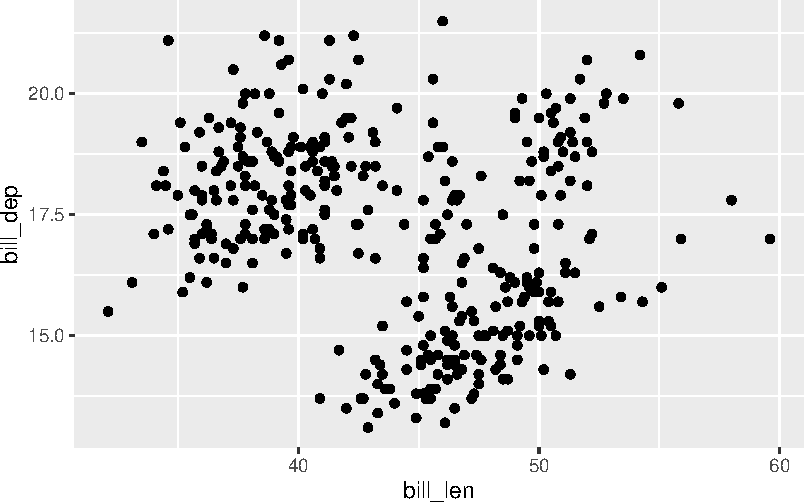
\includegraphics[keepaspectratio]{lab-4_files/figure-pdf/unnamed-chunk-2-1.pdf}}

Add the following code chunk options, one at a time, and set each to
\texttt{false} and then to \texttt{true}. After each value, render your
document and observe its effect. Ultimately, choose the values that are
the most appropriate for this code chunk. Based on the behaviors you
observe, describe what each code chunk option does.

\begin{itemize}
\tightlist
\item
  \texttt{echo}

  \begin{itemize}
  \tightlist
  \item
    When echo = true, the code is shown in the document, whereas when
    echo = false, the code is hidden and only the output (the graph) is
    shown.
  \end{itemize}
\item
  \texttt{warning}

  \begin{itemize}
  \tightlist
  \item
    When warning = true, the warning message is shown in the document,
    where as when warning is false, it hides the warning messages.
  \end{itemize}
\item
  \texttt{eval}

  \begin{itemize}
  \tightlist
  \item
    when eval is true, the document runs the code, when eval is false,
    the document doesn't run the code
  \end{itemize}
\end{itemize}

\subsection{Question 3}\label{question-3}

\begin{enumerate}
\def\labelenumi{\alph{enumi}.}
\item
  You have the following code chunk again.

\begin{Shaded}
\begin{Highlighting}[]
\FunctionTok{ggplot}\NormalTok{(penguins, }\FunctionTok{aes}\NormalTok{(}\AttributeTok{x =}\NormalTok{ bill\_len, }\AttributeTok{y =}\NormalTok{ bill\_dep)) }\SpecialCharTok{+} 
  \FunctionTok{geom\_point}\NormalTok{()}
\end{Highlighting}
\end{Shaded}

\begin{verbatim}
Warning: Removed 2 rows containing missing values or values outside the scale range
(`geom_point()`).
\end{verbatim}

  \pandocbounded{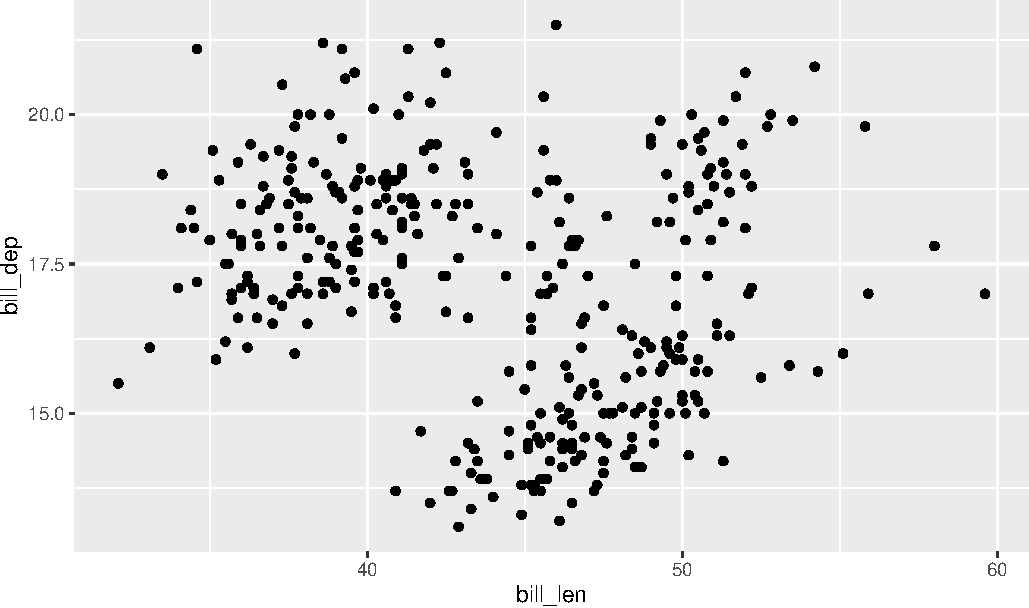
\includegraphics[keepaspectratio]{lab-4_files/figure-pdf/unnamed-chunk-3-1.pdf}}

  Add \texttt{fig-width} and \texttt{fig-asp} as code chunk options. Try
  setting \texttt{fig-width} to values between 1 and 10. Try setting
  \texttt{fig-asp} to values between 0.1 and 1. Re-render the document
  after each value and observe its effect. Ultimately, choose values
  that make the plot look visually pleasing in the rendered document.
  Based on the behavior you observe, describe what each chunk option
  does.
\end{enumerate}

The fig-width option controls how wide the figure appears in the
rendered document, while fig-asp controls the aspect ratio of the
figure, or how tall it appears relative to its width. Increasing
fig-width makes the plot wider, and increasing fig-asp makes the plot
taller.

\begin{enumerate}
\def\labelenumi{\alph{enumi}.}
\item
  You have the following code chunk, but look carefully, it's not
  exactly the same!

\begin{Shaded}
\begin{Highlighting}[]
\FunctionTok{gplot}\NormalTok{(penguins, }\FunctionTok{aes}\NormalTok{(}\AttributeTok{x =}\NormalTok{ bill\_len, }\AttributeTok{y =}\NormalTok{ bill\_dep) }\SpecialCharTok{+} 
  \FunctionTok{geom\_point}\NormalTok{()}
\end{Highlighting}
\end{Shaded}

\begin{verbatim}
Error in parse(text = input): <text>:3:0: unexpected end of input
1: gplot(penguins, aes(x = bill_len, y = bill_dep) + 
2:   geom_point()
  ^
\end{verbatim}

  Add \texttt{error} as a code chunk option and set it to \texttt{false}
  and then set it to \texttt{true}. After each value, render your
  document and observe its effect. Ultimately, choose the value that
  allows you to render your document without altering the code. Based on
  the behavior you observe, describe what this code chunk option does.
\end{enumerate}

The error chunk option controls whether errors in a code chunk stop the
document from rendering. When error = FALSE, the document stops
rendering if an error occurs. When error = TRUE, the document continues
rendering and displays the error message in the output.

\begin{tcolorbox}[enhanced jigsaw, coltitle=black, colbacktitle=quarto-callout-tip-color!10!white, colframe=quarto-callout-tip-color-frame, breakable, leftrule=.75mm, bottomtitle=1mm, left=2mm, opacityback=0, toptitle=1mm, titlerule=0mm, bottomrule=.15mm, title=\textcolor{quarto-callout-tip-color}{\faLightbulb}\hspace{0.5em}{Tip}, arc=.35mm, colback=white, opacitybacktitle=0.6, rightrule=.15mm, toprule=.15mm]

Reading
\href{https://quarto.org/docs/reference/formats/pdf.html\#execution}{the
documentation} might also be hepful.

\end{tcolorbox}

Render, commit, and push one last time. Make sure that you commit and
push all changed documents and your Git pane is completely empty before
proceeding.

\section{Part 2 - Misrepresentation}\label{part-2---misrepresentation}

\subsection{Question 4}\label{question-4}

The following chart was
\href{https://twitter.com/GraphCrimes/status/1566264004288331776}{shared}
by @GraphCrimes on X/Twitter on September 3, 2022.

\begin{center}
\pandocbounded{\includegraphics[keepaspectratio]{images/private-sector.png}}
\end{center}

\begin{enumerate}
\def\labelenumi{\alph{enumi}.}
\tightlist
\item
  What is misleading about this graph?

  \begin{enumerate}
  \def\labelenumii{\alph{enumii}.}
  \tightlist
  \item
    The graph is misleading because the stacked bar segments are not
    clearly scaled or aligned to a consistent baseline, making it
    difficult to accurately compare the proportions across categories.
  \end{enumerate}
\item
  Suppose you wanted to recreate this plot, with improvements to avoid
  its misleading pitfalls from part (a). You would obviously need the
  data from the survey in order to be able to do that. How many
  observations would this data have? How many variables (at least)
  should it have, and what should those variables be?

  \begin{enumerate}
  \def\labelenumii{\alph{enumii}.}
  \tightlist
  \item
    The dataset should contain one observation per respondent for each
    service, in the format of multiple rows per respondent. At minimum,
    it would include variables identifying the respondent, the service
    being evaluated, and their response category (public, private, or
    don't know). There is 1858 participants and 4 categories, so it
    should have a minimum of 7432 individual data points.
  \end{enumerate}
\item
  Load the data for this survey from \texttt{data/survation.csv}.
  Confirm that the data match the percentages from the visualization.
  That is, calculate the percentages of public sector, private sector,
  don't know for each of the services and check that they match the
  percentages from the plot.
\end{enumerate}

\begin{Shaded}
\begin{Highlighting}[]
\CommentTok{\#didn\textquotesingle{}t receive the data file along with the lab so I created the following based on the information on the graph}

\NormalTok{survation }\OtherTok{\textless{}{-}} \FunctionTok{bind\_rows}\NormalTok{(}
  \FunctionTok{tibble}\NormalTok{(}
    \AttributeTok{service =} \StringTok{"Rail"}\NormalTok{,}
    \AttributeTok{response =} \FunctionTok{c}\NormalTok{(}
      \FunctionTok{rep}\NormalTok{(}\StringTok{"Public sector"}\NormalTok{, }\DecValTok{1747}\NormalTok{),}
      \FunctionTok{rep}\NormalTok{(}\StringTok{"Private sector"}\NormalTok{, }\DecValTok{56}\NormalTok{),}
      \FunctionTok{rep}\NormalTok{(}\StringTok{"Don\textquotesingle{}t know"}\NormalTok{, }\DecValTok{55}\NormalTok{)}
\NormalTok{    )}
\NormalTok{  ),}
  \FunctionTok{tibble}\NormalTok{(}
    \AttributeTok{service =} \StringTok{"Water"}\NormalTok{,}
    \AttributeTok{response =} \FunctionTok{c}\NormalTok{(}
      \FunctionTok{rep}\NormalTok{(}\StringTok{"Public sector"}\NormalTok{, }\DecValTok{1747}\NormalTok{),}
      \FunctionTok{rep}\NormalTok{(}\StringTok{"Private sector"}\NormalTok{, }\DecValTok{56}\NormalTok{),}
      \FunctionTok{rep}\NormalTok{(}\StringTok{"Don\textquotesingle{}t know"}\NormalTok{, }\DecValTok{55}\NormalTok{)}
\NormalTok{    )}
\NormalTok{  ),}
  \FunctionTok{tibble}\NormalTok{(}
    \AttributeTok{service =} \StringTok{"Energy"}\NormalTok{,}
    \AttributeTok{response =} \FunctionTok{c}\NormalTok{(}
      \FunctionTok{rep}\NormalTok{(}\StringTok{"Public sector"}\NormalTok{, }\DecValTok{1616}\NormalTok{),}
      \FunctionTok{rep}\NormalTok{(}\StringTok{"Private sector"}\NormalTok{, }\DecValTok{111}\NormalTok{),}
      \FunctionTok{rep}\NormalTok{(}\StringTok{"Don\textquotesingle{}t know"}\NormalTok{, }\DecValTok{131}\NormalTok{)}
\NormalTok{    )}
\NormalTok{  ),}
  \FunctionTok{tibble}\NormalTok{(}
    \AttributeTok{service =} \StringTok{"Royal Mail"}\NormalTok{,}
    \AttributeTok{response =} \FunctionTok{c}\NormalTok{(}
      \FunctionTok{rep}\NormalTok{(}\StringTok{"Public sector"}\NormalTok{, }\DecValTok{1579}\NormalTok{),}
      \FunctionTok{rep}\NormalTok{(}\StringTok{"Private sector"}\NormalTok{, }\DecValTok{130}\NormalTok{),}
      \FunctionTok{rep}\NormalTok{(}\StringTok{"Don\textquotesingle{}t know"}\NormalTok{, }\DecValTok{149}\NormalTok{)}
\NormalTok{    )}
\NormalTok{  )}
\NormalTok{)}

\NormalTok{survation }\SpecialCharTok{\%\textgreater{}\%}
  \FunctionTok{group\_by}\NormalTok{(service, response) }\SpecialCharTok{\%\textgreater{}\%}
  \FunctionTok{summarise}\NormalTok{(}\AttributeTok{n =} \FunctionTok{n}\NormalTok{(), }\AttributeTok{.groups =} \StringTok{"drop"}\NormalTok{) }\SpecialCharTok{\%\textgreater{}\%}
  \FunctionTok{group\_by}\NormalTok{(service) }\SpecialCharTok{\%\textgreater{}\%}
  \FunctionTok{mutate}\NormalTok{(}\AttributeTok{percent =} \FunctionTok{round}\NormalTok{(n }\SpecialCharTok{/} \FunctionTok{sum}\NormalTok{(n) }\SpecialCharTok{*} \DecValTok{100}\NormalTok{, }\DecValTok{0}\NormalTok{)) }\SpecialCharTok{\%\textgreater{}\%}
  \FunctionTok{arrange}\NormalTok{(service, }\FunctionTok{desc}\NormalTok{(percent))}
\end{Highlighting}
\end{Shaded}

\begin{verbatim}
# A tibble: 12 x 4
# Groups:   service [4]
   service    response           n percent
   <chr>      <chr>          <int>   <dbl>
 1 Energy     Public sector   1616      87
 2 Energy     Don't know       131       7
 3 Energy     Private sector   111       6
 4 Rail       Public sector   1747      94
 5 Rail       Don't know        55       3
 6 Rail       Private sector    56       3
 7 Royal Mail Public sector   1579      85
 8 Royal Mail Don't know       149       8
 9 Royal Mail Private sector   130       7
10 Water      Public sector   1747      94
11 Water      Don't know        55       3
12 Water      Private sector    56       3
\end{verbatim}

Please note that the value are consistent with the data from the plot as
the csv datasheet is missing.

\subsection{Question 5}\label{question-5}

Create an improved version of the visualization. Your improved
visualization:

\begin{itemize}
\item
  should also be a stacked bar chart with services on the y-axis,
  presented in the same order as the original plot, and services to
  create the segments of the plot, and presented in the same order as
  the original plot
\item
  should have the same legend location
\item
  should have the same title and caption
\item
  does not need to have a bolded title or a gray background
\end{itemize}

How does the improved visualization look different than the original?
Does it send a different message at a first glance?

\begin{Shaded}
\begin{Highlighting}[]
\NormalTok{survation }\SpecialCharTok{\%\textgreater{}\%}
  \FunctionTok{group\_by}\NormalTok{(service, response) }\SpecialCharTok{\%\textgreater{}\%}
  \FunctionTok{summarise}\NormalTok{(}\AttributeTok{n =} \FunctionTok{n}\NormalTok{(), }\AttributeTok{.groups =} \StringTok{"drop"}\NormalTok{) }\SpecialCharTok{\%\textgreater{}\%}
  \FunctionTok{group\_by}\NormalTok{(service) }\SpecialCharTok{\%\textgreater{}\%}
  \FunctionTok{mutate}\NormalTok{(}\AttributeTok{percent =}\NormalTok{ n }\SpecialCharTok{/} \FunctionTok{sum}\NormalTok{(n) }\SpecialCharTok{*} \DecValTok{100}\NormalTok{) }\SpecialCharTok{\%\textgreater{}\%}
  \FunctionTok{mutate}\NormalTok{(}
    \AttributeTok{service =} \FunctionTok{factor}\NormalTok{(service, }\AttributeTok{levels =} \FunctionTok{c}\NormalTok{(}\StringTok{"Rail"}\NormalTok{, }\StringTok{"Water"}\NormalTok{, }\StringTok{"Energy"}\NormalTok{, }\StringTok{"Royal Mail"}\NormalTok{)),}
    \AttributeTok{response =} \FunctionTok{factor}\NormalTok{(response,}
                      \AttributeTok{levels =} \FunctionTok{c}\NormalTok{(}\StringTok{"Public sector"}\NormalTok{, }\StringTok{"Private sector"}\NormalTok{, }\StringTok{"Don\textquotesingle{}t know"}\NormalTok{))}
\NormalTok{  ) }\SpecialCharTok{\%\textgreater{}\%}
  \FunctionTok{ggplot}\NormalTok{(}\FunctionTok{aes}\NormalTok{(}\AttributeTok{x =}\NormalTok{ percent, }\AttributeTok{y =}\NormalTok{ service, }\AttributeTok{fill =}\NormalTok{ response)) }\SpecialCharTok{+}
  \FunctionTok{geom\_col}\NormalTok{(}\AttributeTok{width =} \FloatTok{0.5}\NormalTok{) }\SpecialCharTok{+}
  \FunctionTok{geom\_text}\NormalTok{(}\FunctionTok{aes}\NormalTok{(}\AttributeTok{label =} \FunctionTok{paste0}\NormalTok{(}\FunctionTok{round}\NormalTok{(percent), }\StringTok{"\%"}\NormalTok{)),}
            \AttributeTok{position =} \FunctionTok{position\_stack}\NormalTok{(}\AttributeTok{vjust =} \FloatTok{0.5}\NormalTok{),}
            \AttributeTok{color =} \StringTok{"white"}\NormalTok{,}
            \AttributeTok{size =} \DecValTok{4}\NormalTok{) }\SpecialCharTok{+}
  \FunctionTok{scale\_fill\_manual}\NormalTok{(}
    \AttributeTok{values =} \FunctionTok{c}\NormalTok{(}
      \StringTok{"Public sector"} \OtherTok{=} \StringTok{"\#006697"}\NormalTok{,}
      \StringTok{"Private sector"} \OtherTok{=} \StringTok{"\#FF3205"}\NormalTok{,}
      \StringTok{"Don\textquotesingle{}t know"} \OtherTok{=} \StringTok{"gray"}
\NormalTok{    )}
\NormalTok{  ) }\SpecialCharTok{+}
  \FunctionTok{scale\_x\_continuous}\NormalTok{(}
    \AttributeTok{limits =} \FunctionTok{c}\NormalTok{(}\DecValTok{0}\NormalTok{, }\DecValTok{100}\NormalTok{),}
    \AttributeTok{breaks =} \FunctionTok{seq}\NormalTok{(}\DecValTok{0}\NormalTok{, }\DecValTok{100}\NormalTok{, }\DecValTok{20}\NormalTok{),}
    \AttributeTok{labels =}\NormalTok{ \textbackslash{}(x) }\FunctionTok{paste0}\NormalTok{(x, }\StringTok{"\%"}\NormalTok{)}
\NormalTok{  ) }\SpecialCharTok{+}
  \FunctionTok{labs}\NormalTok{(}
    \AttributeTok{title =} \StringTok{"Q4. Do you think the following services should be run in the private}\SpecialCharTok{\textbackslash{}n}\StringTok{sector or the public sector?"}\NormalTok{,}
    \AttributeTok{x =} \StringTok{"Percentage"}\NormalTok{,}
    \AttributeTok{y =} \ConstantTok{NULL}\NormalTok{,}
    \AttributeTok{fill =} \ConstantTok{NULL}\NormalTok{,}
    \AttributeTok{caption =} \StringTok{"Base: All Respondents Unweighted Total: Total=1858"}
\NormalTok{  ) }\SpecialCharTok{+}
  \FunctionTok{theme\_minimal}\NormalTok{() }\SpecialCharTok{+}
  \FunctionTok{theme}\NormalTok{(}
    \AttributeTok{legend.position =} \StringTok{"bottom"}\NormalTok{,}
    \AttributeTok{panel.grid.major.y =} \FunctionTok{element\_blank}\NormalTok{(),}
    \AttributeTok{panel.grid.minor =} \FunctionTok{element\_blank}\NormalTok{()}
\NormalTok{  )}
\end{Highlighting}
\end{Shaded}

\pandocbounded{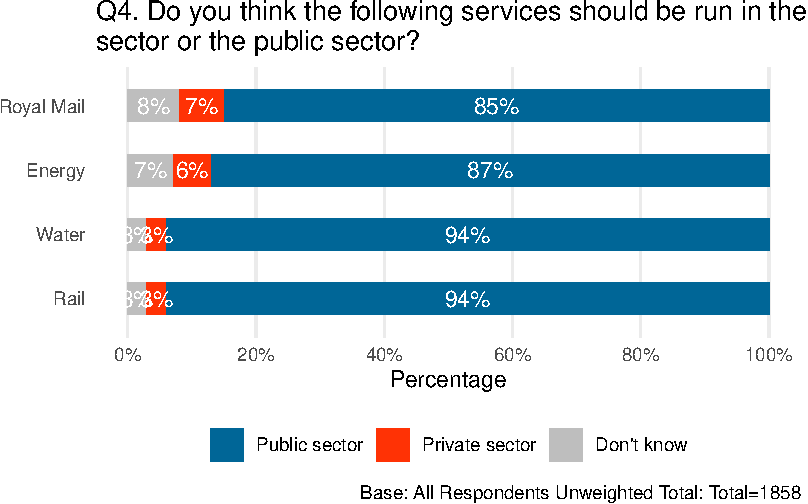
\includegraphics[keepaspectratio]{lab-4_files/figure-pdf/unnamed-chunk-6-1.pdf}}

The improved graph incorporates a more accurate scaling and thus sends a
different message by visualizing how the vast majority of people have a
strong preferences for these services to be ran by the public sector.

\begin{tcolorbox}[enhanced jigsaw, coltitle=black, colbacktitle=quarto-callout-tip-color!10!white, colframe=quarto-callout-tip-color-frame, breakable, leftrule=.75mm, bottomtitle=1mm, left=2mm, opacityback=0, toptitle=1mm, titlerule=0mm, bottomrule=.15mm, title=\textcolor{quarto-callout-tip-color}{\faLightbulb}\hspace{0.5em}{Tip}, arc=.35mm, colback=white, opacitybacktitle=0.6, rightrule=.15mm, toprule=.15mm]

Use \texttt{\textbackslash{}n} to add a line break to your title. And
note that since the title is very long, it might run off the page in
your code. That's ok!

Additionally, the colors used in the plot are \texttt{gray},
\texttt{\#FF3205}, and \texttt{\#006697}.

\end{tcolorbox}

Render, commit, and push one last time. Make sure that you commit and
push all changed documents and your Git pane is completely empty before
proceeding.

\section{Part 3 - DatasauRus}\label{part-3---datasaurus}

The data frame you will be working with in this part is called
\texttt{datasaurus\_dozen} and it's in the \textbf{datasauRus} package.
This single data frame contains 13 datasets, designed to show us why
data visualization is important and how summary statistics alone can be
misleading. The different datasets are marked by the \texttt{dataset}
variable, as shown in Figure~\ref{fig-datasaurus}.

\begin{figure}

\centering{

\includegraphics[width=4.5in,height=\textheight,keepaspectratio]{images/datasaurus-dozen.png}

}

\caption{\label{fig-datasaurus}The `datasaurus\_dozen` data frame stacks
13 datasets on top of each other. This figure shows the first three
datasets.}

\end{figure}%

\begin{tcolorbox}[enhanced jigsaw, coltitle=black, colbacktitle=quarto-callout-note-color!10!white, colframe=quarto-callout-note-color-frame, breakable, leftrule=.75mm, bottomtitle=1mm, left=2mm, opacityback=0, toptitle=1mm, titlerule=0mm, bottomrule=.15mm, title=\textcolor{quarto-callout-note-color}{\faInfo}\hspace{0.5em}{Note}, arc=.35mm, colback=white, opacitybacktitle=0.6, rightrule=.15mm, toprule=.15mm]

If it's confusing that the data frame is called
\texttt{datasaurus\_dozen} when it contains 13 datasets, you're not
alone! Have you heard of a
\href{https://www.mentalfloss.com/article/32259/why-bakers-dozen-13}{baker's
dozen}?

\end{tcolorbox}

Here is a peek at the top 10 rows of the dataset:

\begin{Shaded}
\begin{Highlighting}[]
\NormalTok{datasaurus\_dozen}
\end{Highlighting}
\end{Shaded}

\begin{verbatim}
# A tibble: 1,846 x 3
   dataset     x     y
   <chr>   <dbl> <dbl>
 1 dino     55.4  97.2
 2 dino     51.5  96.0
 3 dino     46.2  94.5
 4 dino     42.8  91.4
 5 dino     40.8  88.3
 6 dino     38.7  84.9
 7 dino     35.6  79.9
 8 dino     33.1  77.6
 9 dino     29.0  74.5
10 dino     26.2  71.4
# i 1,836 more rows
\end{verbatim}

\subsection{Question 6}\label{question-6}

In a single pipeline, calculate the mean of \texttt{x}, mean of
\texttt{y}, standard deviation of \texttt{x}, standard deviation of
\texttt{y}, and the correlation between \texttt{x} and \texttt{y} for
each level of the \texttt{dataset} variable. Then, in 1-2 sentences,
comment on how these summary statistics compare across groups
(datasets).

\begin{Shaded}
\begin{Highlighting}[]
\NormalTok{datasaurus\_dozen }\SpecialCharTok{\%\textgreater{}\%}
  \FunctionTok{group\_by}\NormalTok{(dataset) }\SpecialCharTok{\%\textgreater{}\%}
  \FunctionTok{summarise}\NormalTok{(}
    \AttributeTok{mean\_x =} \FunctionTok{mean}\NormalTok{(x),}
    \AttributeTok{mean\_y =} \FunctionTok{mean}\NormalTok{(y),}
    \AttributeTok{sd\_x =} \FunctionTok{sd}\NormalTok{(x),}
    \AttributeTok{sd\_y =} \FunctionTok{sd}\NormalTok{(y),}
    \AttributeTok{correlation =} \FunctionTok{cor}\NormalTok{(x, y)}
\NormalTok{  ) }\SpecialCharTok{\%\textgreater{}\%}
  \FunctionTok{print}\NormalTok{(}\AttributeTok{n =} \DecValTok{13}\NormalTok{)}
\end{Highlighting}
\end{Shaded}

\begin{verbatim}
# A tibble: 13 x 6
   dataset    mean_x mean_y  sd_x  sd_y correlation
   <chr>       <dbl>  <dbl> <dbl> <dbl>       <dbl>
 1 away         54.3   47.8  16.8  26.9     -0.0641
 2 bullseye     54.3   47.8  16.8  26.9     -0.0686
 3 circle       54.3   47.8  16.8  26.9     -0.0683
 4 dino         54.3   47.8  16.8  26.9     -0.0645
 5 dots         54.3   47.8  16.8  26.9     -0.0603
 6 h_lines      54.3   47.8  16.8  26.9     -0.0617
 7 high_lines   54.3   47.8  16.8  26.9     -0.0685
 8 slant_down   54.3   47.8  16.8  26.9     -0.0690
 9 slant_up     54.3   47.8  16.8  26.9     -0.0686
10 star         54.3   47.8  16.8  26.9     -0.0630
11 v_lines      54.3   47.8  16.8  26.9     -0.0694
12 wide_lines   54.3   47.8  16.8  26.9     -0.0666
13 x_shape      54.3   47.8  16.8  26.9     -0.0656
\end{verbatim}

\begin{tcolorbox}[enhanced jigsaw, coltitle=black, colbacktitle=quarto-callout-tip-color!10!white, colframe=quarto-callout-tip-color-frame, breakable, leftrule=.75mm, bottomtitle=1mm, left=2mm, opacityback=0, toptitle=1mm, titlerule=0mm, bottomrule=.15mm, title=\textcolor{quarto-callout-tip-color}{\faLightbulb}\hspace{0.5em}{Tip}, arc=.35mm, colback=white, opacitybacktitle=0.6, rightrule=.15mm, toprule=.15mm]

There are 13 groups but \texttt{tibble}s only print out 10 rows by
default. Add \texttt{print(n\ =\ 13)} as the last step of your pipeline
to display all rows.

\end{tcolorbox}

The summary statistics are nearly identical across all datasets, with
the same means and standard deviations for both x and y, and very
similar correlation values. Despite this, the datasets represent very
different patterns when visualized, demonstrating that relying only on
summary statistics can be misleading.

\subsection{Question 7}\label{question-7}

Create a scatterplot of \texttt{y} versus \texttt{x} and color and facet
it by \texttt{dataset}. Then, in 1-2 sentences, how these plots compare
across groups (datasets). How does your response in this question
compare to your response to the previous question and what does this say
about using visualizations and summary statistics when getting to know a
dataset?

\begin{Shaded}
\begin{Highlighting}[]
\NormalTok{datasaurus\_dozen }\SpecialCharTok{\%\textgreater{}\%}
  \FunctionTok{ggplot}\NormalTok{(}\FunctionTok{aes}\NormalTok{(}\AttributeTok{x =}\NormalTok{ x, }\AttributeTok{y =}\NormalTok{ y, }\AttributeTok{color =}\NormalTok{ dataset)) }\SpecialCharTok{+}
  \FunctionTok{geom\_point}\NormalTok{(}\AttributeTok{show.legend =} \ConstantTok{FALSE}\NormalTok{) }\SpecialCharTok{+}
  \FunctionTok{facet\_wrap}\NormalTok{(}\SpecialCharTok{\textasciitilde{}}\NormalTok{ dataset) }\SpecialCharTok{+}
  \FunctionTok{labs}\NormalTok{(}
    \AttributeTok{title =} \StringTok{"Datasaurus Dozen: Same stats, different shapes"}\NormalTok{,}
    \AttributeTok{x =} \StringTok{"x"}\NormalTok{,}
    \AttributeTok{y =} \StringTok{"y"}
\NormalTok{  ) }\SpecialCharTok{+}
  \FunctionTok{theme\_minimal}\NormalTok{()}
\end{Highlighting}
\end{Shaded}

\pandocbounded{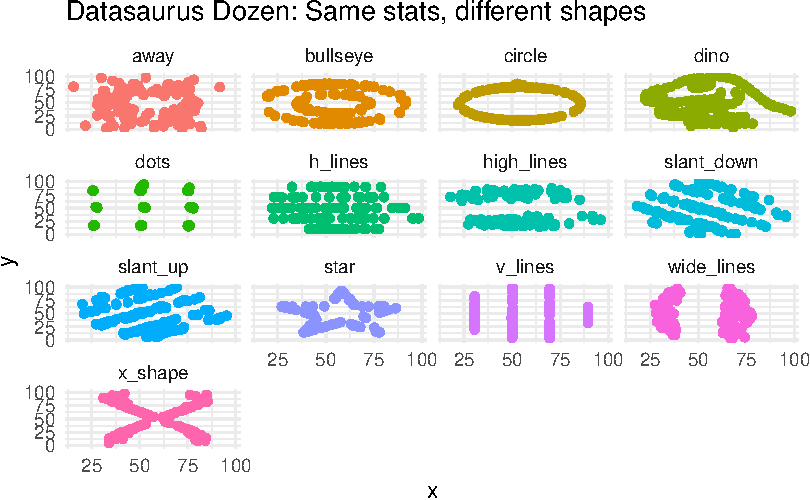
\includegraphics[keepaspectratio]{lab-4_files/figure-pdf/unnamed-chunk-9-1.pdf}}

The scatterplots differ dramatically across datasets, forming distinct
shapes such as lines, curves, and even recognizable figures like a
dinosaur and a star, despite having nearly identical summary statistics.
Compared to the previous question, this shows that while summary
statistics suggest the datasets are similar, visualizations reveal
important structural differences, highlighting the importance of using
both when analyzing data.

\begin{tcolorbox}[enhanced jigsaw, coltitle=black, colbacktitle=quarto-callout-tip-color!10!white, colframe=quarto-callout-tip-color-frame, breakable, leftrule=.75mm, bottomtitle=1mm, left=2mm, opacityback=0, toptitle=1mm, titlerule=0mm, bottomrule=.15mm, title=\textcolor{quarto-callout-tip-color}{\faLightbulb}\hspace{0.5em}{Tip}, arc=.35mm, colback=white, opacitybacktitle=0.6, rightrule=.15mm, toprule=.15mm]

When you both color and facet by the same variable, you'll end up with a
redundant legend. Turn off the legend by adding
\texttt{show.legend\ =\ FALSE} to the geom creating the legend.

\end{tcolorbox}

Render, commit, and push one last time. Make sure that you commit and
push all changed documents and your Git pane is completely empty before
proceeding.

\subsection{Grading}\label{grading}

The lab is graded out of a total of 28 points.

You can earn up to 4 points on each question:

\begin{itemize}
\item
  4: Response shows excellent understanding and addresses all or almost
  all of the rubric items.
\item
  3: Response shows good understanding and addresses most of the rubric
  items.
\item
  2: Response shows understanding and addresses a majority of the rubric
  items.
\item
  1: Response shows effort and misses many of the rubric items.
\item
  0: Response does not show sufficient effort or understanding and/or is
  largely incomplete.
\end{itemize}




\end{document}
